\section{Local zeros and small derivatives}
\label{sec:local-roots}
\subsection{Local zero counts}\label{sec:local-root-count}
We will use the Hanson--Wright inequality of Rudelson--Vershynin
\cite[Theorem 1.1]{RudelsonVershynin2013}: if $\xi$ is a random vector
with independent centered real coordinates whose
$\psi_2$ norm is at most $\Lambda$, $M$ is a real matrix and $t>0$, then
\[
 \Prob\{|\xi^TM\xi-\mathbb E\xi^TM\xi|>t\}
 \le2\exp\left[-c_{\rm HW}\min\left\{
 \frac{t^2}{\Lambda^4\|M\|_{\rm HS}^2},\frac{t}{\Lambda^2\|M\|}\right\}\right],
\]
where $c_{\rm HW}>0$ is an absolute constant.
Rudelson and Vershynin use the moment convention for $\psi_2$, and signs
satisfy both it and the equivalent exponential-moment convention with
$\Lambda=2$, since $p^{-1/2}(\mathbb E|\epsilon_k|^p)^{1/p}=p^{-1/2}\le2$
for $p\ge1$ and $\mathbb E\exp(\epsilon_k^2/2^2)=e^{1/4}\le2$.
Hence, for independent uniform signs $\epsilon=(\epsilon_0,\dots,\epsilon_N)$,
a real $(N+1)\times(N+1)$ matrix $M$ and $t>0$,
\begin{equation}
 \Prob\{|\epsilon^TM\epsilon-\mathbb E\epsilon^TM\epsilon|>t\}
 \le2\exp\left[-c_{\rm HW}\min\left\{
 \frac{t^2}{16\|M\|_{\rm HS}^2},\frac{t}{4\|M\|}\right\}\right].
 \label{eq:HW-signs}
\end{equation}

We first bound the local zero counts when the coefficients are independent
signs times bounded amplitudes, and then we specialize this bound to signs.

\begin{lemma}[Local zero counts for bounded amplitudes]
\label{lem:local-counts-general}
Fix $K\ge2$, $B\ge1$ and $\tfrac12\le\eta\le1$, and put
\[
 A(B,\eta)=\max\left(1,\frac{1024\pi B^2}{c_{\rm HW}\eta}\right),\qquad
 t_N(B,\eta)=\frac{A(B,\eta)\log N}{N},
\]
\[
 C_1(K,B,\eta)=\frac{4A(B,\eta)+4K+4+\log B}{\log2}.
\]
Let $N\ge e$ with $t_N(B,\eta)\le1$.
Let $\epsilon_0,\dots,\epsilon_N$ be independent uniform signs, and let
$a_0,\dots,a_N$ be real or complex random variables, independent of the
signs, with $|a_k|\le B$ for every $k$.
Let $\mathcal E$ be an event determined by $a_0,\dots,a_N$ on which
\[
 \sum_{k=0}^N|a_k|^2\ge\eta(N+1),
\]
and put $P_N(z)=\sum_{k=0}^N\epsilon_ka_kz^k$.
Then the probability that $\mathcal E$ occurs and some disk
\[
 \{z:|z-z_0|\le2K/N\},\qquad ||z_0|-1|\le1/N,
\]
contains more than $C_1(K,B,\eta)\log N$ zeros of $P_N$ is at most $N^{-3}$.
\end{lemma}

\begin{proof}
The idea is to show that the mean of $|P_N|^2$ over each arc of a fine
angular grid is at least half its conditional expectation, and then to
apply Jensen's formula at a point of the arc at which $|P_N|$ is large.

We condition on $a_0,\dots,a_N$ and assume that $\mathcal E$ occurs, so
that the signs remain independent and uniform. We take
$J=\lceil2\pi/t_N(B,\eta)\rceil$ equally spaced angular centers, with the
closed arc of radian length $2t_N(B,\eta)$ around each center.
Since $t_N(B,\eta)\le1<\pi$, every such arc $I$ has
$\mu(I)=t_N(B,\eta)/\pi$, and since $A(B,\eta)\ge1$ and $\log N\ge1$,
\[
 J\le\frac{2\pi}{t_N(B,\eta)}+1=\frac{2\pi N}{A(B,\eta)\log N}+1
 \le2\pi N+1\le8N.
\]
For each such arc $I$, the conditional real Gram matrix is defined by
\[
 (A_I)_{jk}=\int_I\Re\bigl(a_j\overline{a_k}e^{i(j-k)\theta}\bigr)\dd\mu(\theta),
 \qquad 0\le j,k\le N.
\]
For every real vector $x$, since the $x_k$ are real and by Parseval's
identity on the whole circle, we have
\begin{align*}
 0\le x^TA_Ix
 &=\int_I\left|\sum_{k=0}^Nx_ka_ke^{ik\theta}\right|^2\dd\mu(\theta)
 \le\int\left|\sum_{k=0}^Nx_ka_ke^{ik\theta}\right|^2\dd\mu(\theta)\\
 &=\sum_{k=0}^Nx_k^2|a_k|^2\le B^2\|x\|^2.
\end{align*}
It follows that the eigenvalues of the real symmetric matrix $A_I$ lie in
$[0,B^2]$, and since they are nonnegative, we have
\begin{gather*}
 \|A_I\|\le B^2,\qquad
 \|A_I\|_{\rm HS}^2\le\|A_I\|\operatorname{tr}A_I\le B^2\operatorname{tr}A_I,\\
 \operatorname{tr}A_I=\mu(I)\sum_{k=0}^N|a_k|^2\ge\eta(N+1)\mu(I)
 =\frac{\eta(N+1)t_N(B,\eta)}{\pi},
\end{gather*}
where the trace identity follows from $(A_I)_{kk}=|a_k|^2\mu(I)$, and the
inequality after it from $\mathcal E$.
Taking $x=\epsilon$ in the identity above and using
$\mathbb E\epsilon_j\epsilon_k=\mathbf 1\{j=k\}$, we obtain
\[
 Q_I:=\int_I|P_N(e^{i\theta})|^2\dd\mu(\theta)=\epsilon^TA_I\epsilon,\qquad
 \mathbb E_\epsilon Q_I=\operatorname{tr}A_I.
\]
If $Q_I<\tfrac12\operatorname{tr}A_I$, then
$|Q_I-\mathbb E_\epsilon Q_I|>\tfrac12\operatorname{tr}A_I$.
By \eqref{eq:HW-signs} with $M=A_I$ and $t=\tfrac12\operatorname{tr}A_I$,
and the bounds above, we have
\begin{align*}
 \Prob_\epsilon\{Q_I<\tfrac12\operatorname{tr}A_I\}
 &\le2\exp\left[-c_{\rm HW}\min\left\{
   \frac{(\operatorname{tr}A_I)^2}{64\|A_I\|_{\rm HS}^2},
   \frac{\operatorname{tr}A_I}{8\|A_I\|}\right\}\right]\\
 &\le2\exp\left[-c_{\rm HW}\min\left\{
   \frac{\operatorname{tr}A_I}{64B^2},
   \frac{\operatorname{tr}A_I}{8B^2}\right\}\right]
 =2\exp\left[-\frac{c_{\rm HW}\operatorname{tr}A_I}{64B^2}\right]\\
 &\le2\exp\left[-\frac{c_{\rm HW}\eta(N+1)A(B,\eta)\log N}{64\pi B^2N}\right]
 \le2e^{-16\log N}=2N^{-16},
\end{align*}
where the last inequality holds since
$A(B,\eta)\ge1024\pi B^2/(c_{\rm HW}\eta)$.
By the union bound over the at most $8N$ arcs, we get
\[
 \Prob_\epsilon\{Q_I<\tfrac12\operatorname{tr}A_I
 \text{ for some arc }I\}
 \le(8N)(2N^{-16})=16N^{-15}\le N^{-3}.
\]
Taking the expectation over $a_0,\dots,a_N$ on $\mathcal E$, we see that
the probability that $\mathcal E$ occurs and some arc has
$Q_I<\tfrac12\operatorname{tr}A_I$ is at most $N^{-3}$.

It remains to bound the number of zeros when $\mathcal E$ occurs and
every arc has $Q_I\ge\tfrac12\operatorname{tr}A_I$.
In this case, averaging over each closed arc and using the lower bound on
$\operatorname{tr}A_I$, we get
\[
 \max_{\theta\in I}|P_N(e^{i\theta})|^2\ge\frac{Q_I}{\mu(I)}
 \ge\frac{\operatorname{tr}A_I}{2\mu(I)}\ge\frac{\eta(N+1)}2.
\]
By continuity, there exists $z_1=e^{i\theta_1}$ on the arc such that
$|P_N(z_1)|^2\ge\eta(N+1)/2$.
Now let $||z_0|-1|\le1/N$.
Then the angular center nearest to $z_0/|z_0|$ is at angular distance at
most $\pi/J\le t_N(B,\eta)/2$ from it, and such a point $z_1$ on its arc
is at angular distance at most $t_N(B,\eta)$ from the center, so that
$|z_0/|z_0|-z_1|\le3t_N(B,\eta)/2$, since a chord is at most its arc.
Let $R=(2K+1)/N+2t_N(B,\eta)$. For $|z-z_0|\le2K/N$, since
$\bigl|z_0-z_0/|z_0|\bigr|=||z_0|-1|\le1/N$, we have
\[
 |z-z_1|\le|z-z_0|+\bigl|z_0-z_0/|z_0|\bigr|+\bigl|z_0/|z_0|-z_1\bigr|
 \le\frac{2K}N+\frac1N+\frac{3t_N(B,\eta)}2<R,
\]
so that the target disk lies strictly within $\{|z-z_1|<R\}$.
For $|z-z_1|\le2R$ we have $|z|\le1+2R$, and hence
\[
 |P_N(z)|\le\sum_{k=0}^N|a_k||z|^k\le B(N+1)(1+2R)^N\le B(N+1)e^{2NR}.
\]
Let $n(s)$ denote the number of zeros of $P_N$ in $|z-z_1|\le s$.
Since $P_N(z_1)\ne0$, Jensen's formula applies on the disk $|z-z_1|\le2R$,
and using $2NR=4K+2+4A(B,\eta)\log N$ we get
\begin{align*}
 &\#\{\alpha:|\alpha-z_1|<R\}
 \le n(R)\le\frac1{\log2}\int_R^{2R}\frac{n(s)}s\dd s\\
 &\qquad\le\frac{\max_{|z-z_1|=2R}\log|P_N(z)|-\log|P_N(z_1)|}{\log2}\\
 &\qquad\le\frac{\log\bigl(B(N+1)e^{2NR}\bigr)
   -\tfrac12\log\bigl(\eta(N+1)/2\bigr)}{\log2}\\
 &\qquad=\frac{\tfrac12\log(N+1)+\log B+\tfrac12\log(2/\eta)+2NR}{\log2}\\
 &\qquad=\frac{\tfrac12\log(N+1)+\log B+\tfrac12\log(2/\eta)
   +4K+2+4A(B,\eta)\log N}{\log2}\\
 &\qquad\le\frac{\log N+(4K+3+\log B)\log N+4A(B,\eta)\log N}{\log2}
 =C_1(K,B,\eta)\log N.
\end{align*}
The second inequality is the zero-count step of
\cite[\S8.21]{Titchmarsh1939}, the third is Jensen's formula
\cite[\S3.61]{Titchmarsh1939} for $P_N(z_1+z)$, and the last uses
$\tfrac12\log(N+1)\le\log N$ for $N\ge2$,
$\tfrac12\log(2/\eta)\le\tfrac12\log4=\log2$ for $\eta\ge\tfrac12$, and
$\log B+\log2+4K+2\le(4K+3+\log B)\log N$, which holds for
$\log N\ge1$ since $\log B\ge0$ and $\log2<1$.
Since the containment is strict, this count includes the zeros on the
boundary of the target disk, and since the angular cover is finite and
does not depend on $z_0$, the bound holds for every admissible center
$z_0$ at once.
\end{proof}

\begin{lemma}[Local zero counts]\label{lem:local-counts}
Fix $K\ge2$ and take $N$ sufficiently large.
Except on an event of probability at most $N^{-3}$, every disk
\[
 \{z:|z-z_0|\le2K/N\},\qquad ||z_0|-1|\le1/N,
\]
contains at most $C(K)\log N$ zeros of $f_N$.
\end{lemma}

The local-count constant is computed in Section~\ref{app:const-local}.

\begin{proof}
We apply Lemma~\ref{lem:local-counts-general} with $a_k=1$ for every $k$,
$B=1$, $\eta=1$ and $\mathcal E=\Omega$, which we may do since
$\sum_{k=0}^N|a_k|^2=N+1$.
Then $P_N=f_N$, and since $\log1=0$, the constants of that lemma are
\begin{align*}
 A(1,1)&=\max(1,1024\pi/c_{\rm HW})=A,\qquad
 t_N(1,1)=\frac{A\log N}N=t_N,\\
 C_1(K,1,1)&=\frac{4A+4K+4}{\log2}=C_1(K),
\end{align*}
which are the constants of Section~\ref{app:const-local}.
The conditions $N\ge e$ and $t_N\le1$ hold for all sufficiently large
$N$, since $t_N\to0$.
This proves the lemma with $C(K)=C_1(K)$.
\end{proof}

\subsection{Derivative detection and small-ball estimates}\label{sec:derivative-detection}
In this subsection we fix $K\ge2$, let $L=N^{1/64}$, and consider the
annulus $||z|-1|\le K/N$.

\begin{lemma}[Second derivative]\label{lem:second-derivative}
For every $N\ge\max\{2,(K+1)/3\}$, outside an event of probability at most
$N^{-10}$,
\begin{equation}
 \sup_{|z|\le1+(K+1)/N}|f_N''(z)|
 \le C(K)N^{5/2}\sqrt{\log N},
                                                        \label{eq:sign-second-derivative}
\end{equation}
and one can take $C(K)=100e^{K+4}$.
\end{lemma}

\begin{proof}
We first bound $f_N''$ at finitely many points of the circle
$|z|=1+(K+1)/N$ by Hoeffding's inequality, then pass to the whole circle
using a deterministic bound on $f_N'''$, and finally to the disk by the
maximum principle.
Bounds of this order for the supremum of a random trigonometric
polynomial go back to Salem and Zygmund \cite[Chapter~6]{Kahane1985}.

We choose $\lceil N^3\rceil\le2N^3$ equally spaced points on the boundary
circle, and at each sample $z$ we take
$b=100e^{K+4}N^{5/2}\sqrt{\log N}$.
Since $|z|=1+(K+1)/N$ and $0\le2k-4\le2N$ for $2\le k\le N$, we have
$|z|^{2k-4}\le(1+(K+1)/N)^{2N}\le e^{2K+2}$, and hence
\[
 \sum_{k=2}^Nk^2(k-1)^2|z|^{2k-4}
 \le e^{2K+2}\sum_{k=2}^Nk^4\le2e^{2K+2}N^5.
\]
By Hoeffding's inequality \cite[Theorem~2]{Hoeffding1963}, applied to
both tails,
$\Prob\{|\sum_k\epsilon_kc_k|\ge t\}\le2\exp[-t^2/(2\sum_kc_k^2)]$ for real
numbers $c_k$ and $t>0$.
Applying this real bound to the real and imaginary parts
$\Re f_N''(z)=\sum_{k=2}^N\epsilon_kk(k-1)\Re(z^{k-2})$ and
$\Im f_N''(z)=\sum_{k=2}^N\epsilon_kk(k-1)\Im(z^{k-2})$, whose squared
coefficients are at most $k^2(k-1)^2|z|^{2k-4}$, we get
\begin{align*}
 \Prob\{|f_N''(z)|\ge b/2\}
 &\le\Prob\Bigl\{|\Re f_N''(z)|\ge\frac b{2\sqrt2}\Bigr\}
   +\Prob\Bigl\{|\Im f_N''(z)|\ge\frac b{2\sqrt2}\Bigr\}\\
 &\le4\exp\left[-\frac{(b/2)^2}
 {4\sum_{k=2}^Nk^2(k-1)^2|z|^{2k-4}}\right]
 \le4\exp\left[-\frac{b^2}{32e^{2K+2}N^5}\right]\\
 &=4\exp\left[-\frac{10000e^6}{32}\log N\right]
 \le4\exp[-100\log N]=4N^{-100},
\end{align*}
where the first step holds since $|f_N''(z)|\ge b/2$ implies that one of
the two parts is at least $b/(2\sqrt2)$ in absolute value.

Since $N\ge(K+1)/3$, the boundary circle has radius $1+(K+1)/N\le4$ and
length at most $8\pi$, so that
each point of it lies within arc length $4\pi/N^3$ of a sample.
Moreover, we have the deterministic bound
\begin{align*}
 \sup_{|z|\le1+(K+1)/N}|f_N'''(z)|
 &\le\sup_{|z|\le1+(K+1)/N}\sum_{k=3}^Nk(k-1)(k-2)|z|^{k-3}\\
 &\le N^3\cdot N\cdot\Bigl(1+\frac{K+1}N\Bigr)^N
 \le e^{K+1}N^4.
\end{align*}
Integrating $f_N'''$ along the arc from a point of the circle to its
nearest sample, we see from this bound that the interpolation error is at
most $4\pi e^{K+1}N$, which is less than $b/2$ for every $N\ge2$, that is,
\begin{align*}
 \frac{4\pi}{N^3}\sup_{|z|\le1+(K+1)/N}|f_N'''(z)|
 &\le\frac{4\pi}{N^3}e^{K+1}N^4
 =4\pi e^{K+1}N\\
 &<50e^{K+4}N^{5/2}\sqrt{\log N}
 =\frac b2,
\end{align*}
since $4\pi<50e^3\sqrt{\log2}$ and $N^{3/2}\sqrt{\log N}\ge\sqrt{\log2}$.
By the union bound over the samples, the probability that
$|f_N''(z)|\ge b/2$ for some sample $z$ is at most
$(2N^3)(4N^{-100})=8N^{-97}\le N^{-10}$.
Outside this event, every point $\zeta$ of the circle of radius
$1+(K+1)/N$ and its nearest sample $z$ satisfy
$|f_N''(\zeta)|\le|f_N''(z)|+4\pi e^{K+1}N$, so that
$|f_N''|<b/2+b/2=b$ on the circle
$|z|=1+(K+1)/N$, and hence, by the maximum principle, on the disk
$|z|\le1+(K+1)/N$. This proves \eqref{eq:sign-second-derivative} with the
constant $100e^{K+4}$.
\end{proof}

We will use the following inequalities for the block diagonal comparison
of the paired jet covariance in the proof of
Lemma~\ref{lem:small-derivatives}.
Devroye, Mehrabian and Reddad \cite{DevroyeMehrabianReddad2018} give
upper and lower bounds that match up to constant factors for the total
variation distance between Gaussians with equal means, and we need only
an upper bound.

\begin{lemma}[An entropy comparison]\label{lem:entropy}
Let $p,q$ be probability densities, with $p$ absolutely continuous with
respect to $q$, and set
\[
 D(p\Vert q)=\int p\log(p/q),
 \qquad \operatorname{TV}(p,q)=\frac12\int|p-q|.
\]
Then
\[
 \operatorname{TV}(p,q)\le\sqrt{D(p\Vert q)/2}.
\]
For positive-definite covariance matrices $\Sigma,\Sigma_0$ in dimension $d$, let
$G_\Sigma$ and $G_{\Sigma_0}$ be centered Gaussian vectors with these covariances, and set
\[
 R=\Sigma_0^{-1/2}\Sigma\Sigma_0^{-1/2}.
\]
Then
\[
 D\bigl(G_\Sigma\Vert G_{\Sigma_0}\bigr)
 =\frac12\{\operatorname{tr}R-d-\log\det R\}.
\]
If the eigenvalues of $R$ are $1+\eta_1,\ldots,1+\eta_d$ and
$|\eta_j|\le\delta\le1/2$, then
\[
 D\bigl(G_\Sigma\Vert G_{\Sigma_0}\bigr)
 \le\frac12\sum_{j=1}^d\eta_j^2\le\frac d2\delta^2,
\]
\[
 \operatorname{TV}\bigl(G_\Sigma,G_{\Sigma_0}\bigr)
 \le\frac{\sqrt d}{2}\delta.
\]
\end{lemma}

\begin{proof}
The first inequality is Pinsker's inequality
\cite[Lemma~2.5(i)]{Tsybakov2009}. The formula for
$D(G_\Sigma\Vert G_{\Sigma_0})$ is \cite[eq.~(A.23)]{RasmussenWilliams2006}
with zero means and with $\Sigma,\Sigma_0$ in place of the covariances
$\Sigma_0,\Sigma_1$ there, as $\operatorname{tr}(\Sigma_0^{-1}\Sigma)=\operatorname{tr}R$ and
$\log\det(\Sigma_0\Sigma^{-1})=-\log\det R$.
Since the eigenvalues of $R$ are $1+\eta_1,\ldots,1+\eta_d$, we have
$\operatorname{tr}R=\sum_j(1+\eta_j)$ and
$\log\det R=\sum_j\log(1+\eta_j)$, so that
\[
 \operatorname{tr}R-d-\log\det R=\sum_{j=1}^d\{\eta_j-\log(1+\eta_j)\}.
\]
If $|\eta_j|\le\delta\le1/2$, then
$0\le\eta_j-\log(1+\eta_j)\le\eta_j^2$,
since $y-\log(1+y)=\int_0^y t/(1+t)\dd t$, $t/(1+t)$ has the sign of $t$
for $t>-1$, and $|t/(1+t)|\le2|t|$ for $|t|\le1/2$.
It follows that
\[
 D\bigl(G_\Sigma\Vert G_{\Sigma_0}\bigr)
 =\frac12\sum_{j=1}^d\{\eta_j-\log(1+\eta_j)\}
 \le\frac12\sum_{j=1}^d\eta_j^2
 \le\frac d2\delta^2,
\]
and hence, by the first inequality,
\[
 \operatorname{TV}\bigl(G_\Sigma,G_{\Sigma_0}\bigr)
 \le\sqrt{D\bigl(G_\Sigma\Vert G_{\Sigma_0}\bigr)/2}
 \le\sqrt{\frac d4\delta^2}
 =\frac{\sqrt d}{2}\delta.
\]
\end{proof}

\begin{lemma}[Few small derivatives]\label{lem:small-derivatives}
Let $B_{K,N}$ count the roots $\alpha$ of $f_N$ with $||\alpha|-1|\le K/N$
and $|f_N'(\alpha)|<N^{3/2}/L$. For all sufficiently large $N$,
\[
 \Prob\{B_{K,N}>N^{31/32}\}\le N^{-3}+N^{-10}+C(K)N^{-3/8}(\log N)^4.
\]
\end{lemma}

\begin{proof}
The idea is to detect each annular root with a small derivative, outside
two thin sectors around the real axis, at a nearby point of a fixed mesh
at which both $f_N$ and $zf_N'$ are small. We bound the mean and the
variance of the number of such mesh points by one- and two-point Gaussian
approximations, and then the number of roots by Chebyshev's inequality and
the local zero counts, which also bound the roots in the two sectors
directly.

By the Taylor bounds below, at a mesh point $z$ within $h$ of a root,
$|f_N(z)|/\sqrt N$ is at most a constant times
$Nh/L+N^2h^2\sqrt{\log N}$, and for the mean count below both terms must be
at most a constant times $L^{-2}(\log N)^{-1/2}$, which holds when $h$ is
at most a constant times $1/(NL\sqrt{\log N})$. Since a smaller $h$ would
only increase the number of mesh points, we choose a deterministic mesh
with spacing
\[
 h=\frac{c}{NL\sqrt{\log N}},
\]
where $c>0$ is sufficiently small and depends only on $K$. The Taylor
bounds below require $100e^{K+4}c\le1/2$, which also implies that $c\le1$.
The construction in
Section~\ref{app:const-small-derivatives} takes $\lceil2K/(Nh)\rceil+1$
rows, at equally spaced radii from $1-K/N$ to $1+K/N$, and on each row the
same $\lceil8\pi/h\rceil$ equally spaced angles, so that adjacent rows are
at most $h$ apart, and adjacent angles at most $h/4$ apart. Since
$L\sqrt{\log N}/c\ge1$ for $c\le1$ and $N\ge e$, the number of mesh points
satisfies
\begin{align*}
 &\Bigl(\Bigl\lceil\frac{2K}{Nh}\Bigr\rceil+1\Bigr)
 \Bigl\lceil\frac{8\pi}h\Bigr\rceil
 \le\Bigl(\frac{2K}{Nh}+2\Bigr)\Bigl(\frac{8\pi}h+1\Bigr)\\
 &\quad=\Bigl(\frac{2KL\sqrt{\log N}}c+2\Bigr)
   \Bigl(\frac{8\pi NL\sqrt{\log N}}c+1\Bigr)\\
 &\quad\le\frac{(2K+2)L\sqrt{\log N}}c\cdot\frac{(8\pi+1)NL\sqrt{\log N}}c
 \le\frac{53(K+1)}{c^2}NL^2\log N,
\end{align*}
and since $c$ depends only on $K$, the mesh has at most
$C(K)NL^2\log N$ points.

We retain the mesh points $re^{i\theta}$ such that
$\operatorname{dist}(\theta,\pi\mathbb Z)\ge N^{-1/2}$, or equivalently
$\operatorname{dist}(2\theta,2\pi\mathbb Z)\ge2N^{-1/2}$. These are the
angles retained in Section~\ref{sec:h1-rademacher}, and we use them in the
covariance bounds below. Let $\alpha$ be a root with $||\alpha|-1|\le K/N$
and $\operatorname{dist}(\arg\alpha,\pi\mathbb Z)\ge2N^{-1/2}$. We assign
to it the mesh point $z$ on the row nearest to $|\alpha|$ whose angle is
nearest to $\arg\alpha$. Then $\bigl||\alpha|-|z|\bigr|\le h/2$, the angles
of $\alpha$ and $z$ differ by at most $h/8$ modulo $2\pi$, and
$|z|\le1+K/N\le2$ for $N\ge K$, so that, since a chord is at most its arc,
\[
 |\alpha-z|\le\bigl||\alpha|-|z|\bigr|
   +|z|\,\bigl|e^{i\arg\alpha}-e^{i\arg z}\bigr|
 \le\frac h2+2\cdot\frac h8<h.
\]
Moreover, since $h\le1/N\le N^{-1/2}$ for $c\le1$ and $N\ge e$, we have
\[
 \operatorname{dist}(\arg z,\pi\mathbb Z)
 \ge\operatorname{dist}(\arg\alpha,\pi\mathbb Z)-\frac h8
 \ge2N^{-1/2}-N^{-1/2}=N^{-1/2}.
\]
Thus every annular root $\alpha$ with
$\operatorname{dist}(\arg\alpha,\pi\mathbb Z)\ge2N^{-1/2}$ has a retained
mesh point within $h$.

Now let $\alpha$ be such a root with $|f_N'(\alpha)|<N^{3/2}/L$, and let
$z$ be its assigned mesh point.
Since $f_N(\alpha)=0$, by Taylor's theorem with integral remainder at
$\alpha$ we have
\begin{align*}
 \frac{|f_N(z)|}{\sqrt N}
 &=\frac1{\sqrt N}\left|f_N'(\alpha)(z-\alpha)
   +(z-\alpha)^2\int_0^1(1-t)f_N''(\alpha+t(z-\alpha))\dd t\right|\\
 &\le\frac{|f_N'(\alpha)|h}{\sqrt N}
       +\frac{\sup|f_N''|\,h^2}{2\sqrt N}
 \le\frac{Nh}{L}+\frac{C(K)}2N^2h^2\sqrt{\log N}\\
 &=\frac c{L^2\sqrt{\log N}}+\frac{C(K)c^2}{2L^2\sqrt{\log N}}
 \le\frac{C(K)}{L^2\sqrt{\log N}},
\end{align*}
where we used $|z-\alpha|\le h$, $|f_N'(\alpha)|<N^{3/2}/L$ and, on the
event of Lemma~\ref{lem:second-derivative},
\eqref{eq:sign-second-derivative} with $C(K)=100e^{K+4}$, and the last
step holds with the same $C(K)$, since
$c+C(K)c^2/2=c(1+C(K)c/2)\le5c/4\le C(K)$ by $C(K)c\le1/2$ and $c\le1$.
Since $f_N'(z)=f_N'(\alpha)+(z-\alpha)\int_0^1f_N''(\alpha+t(z-\alpha))\dd t$
and $|z|\le2$, we also have
\[
 \frac{|zf_N'(z)|}{N^{3/2}}
 \le2\left(\frac{|f_N'(\alpha)|}{N^{3/2}}
            +\frac{\sup|f_N''|\,h}{N^{3/2}}\right)
 \le\frac{2(1+C(K)c)}L
 \le\frac3L,
\]
since $C(K)c\le1/2$ and, by \eqref{eq:sign-second-derivative},
$\sup|f_N''|\,h/N^{3/2}\le C(K)N^{5/2}\sqrt{\log N}\,h/N^{3/2}=C(K)c/L$.
In both chains the supremum of the second derivative is taken over the
disk $|\zeta|\le1+(K+1)/N$, which contains the segment from $\alpha$ to
$z$, since $\alpha$ and $z$ lie in the convex disk $|\zeta|\le1+K/N$.
Thus the root produces the test
\begin{equation}
 |f_N(z)|/\sqrt N\le u=\frac{C(K)}{L^2\sqrt{\log N}},\qquad
 |zf_N'(z)|/N^{3/2}\le v=3/L.
 \label{eq:annular-mesh-test}
\end{equation}
If a root $\alpha$ is assigned to a mesh point $z$, then, since
$\bigl|z-z/|z|\bigr|=||z|-1|\le K/N$ and $h\le1/N$,
\[
 \bigl|\alpha-z/|z|\bigr|\le|\alpha-z|+\bigl|z-z/|z|\bigr|
 \le h+K/N<2(K+2)/N.
\]
Hence, by Lemma~\ref{lem:local-counts} with $K+2$ in place of $K$, applied
to the disk $\{\zeta:|\zeta-z/|z||\le2(K+2)/N\}$, whose center lies on the
unit circle, at most $C_1(K+2)\log N$ roots are assigned to each cell.

We consider
\[
 W(z)=(W_0(z),W_1(z))=\left(\frac{f_N(z)}{\sqrt N},\frac{zf_N'(z)}{N^{3/2}}\right),
\]
as a real vector with coordinates $\Re W_0(z),\Im W_0(z),\Re W_1(z),\Im W_1(z)$.
For $z=re^{i\theta}$, we have
$W_0(z)=\sum_{k=0}^N\epsilon_kr^ke^{ik\theta}/\sqrt N$ and
$W_1(z)=\sum_{k=0}^N\epsilon_k(k/N)r^ke^{ik\theta}/\sqrt N$, and since the
signs are independent with mean zero and variance one, the real covariance
is
\begingroup
\setlength{\arraycolsep}{1.5pt}
\setlength{\multlinegap}{0pt}
\begin{multline*}
 A_z=\frac1N\sum_{k=0}^Nr^{2k}\\
 \times\begin{pmatrix}
 \cos^2(k\theta)&\cos(k\theta)\sin(k\theta)&
 \frac kN\cos^2(k\theta)&\frac kN\cos(k\theta)\sin(k\theta)\\
 \cos(k\theta)\sin(k\theta)&\sin^2(k\theta)&
 \frac kN\cos(k\theta)\sin(k\theta)&\frac kN\sin^2(k\theta)\\
 \frac kN\cos^2(k\theta)&\frac kN\cos(k\theta)\sin(k\theta)&
 \frac{k^2}{N^2}\cos^2(k\theta)&\frac{k^2}{N^2}\cos(k\theta)\sin(k\theta)\\
 \frac kN\cos(k\theta)\sin(k\theta)&\frac kN\sin^2(k\theta)&
 \frac{k^2}{N^2}\cos(k\theta)\sin(k\theta)&\frac{k^2}{N^2}\sin^2(k\theta)
 \end{pmatrix}.
\end{multline*}
\endgroup
Using
\[
 \cos^2(k\theta)=\frac{1+\cos(2k\theta)}2,\quad
 \sin^2(k\theta)=\frac{1-\cos(2k\theta)}2,\quad
 \cos(k\theta)\sin(k\theta)=\frac{\sin(2k\theta)}2,
\]
we write $A_z=A_z^{(0)}+E_z$, where
\[
 A_z^{(0)}=\frac1{2N}\sum_{k=0}^Nr^{2k}
 \begin{pmatrix}
 1&0&k/N&0\\0&1&0&k/N\\
 k/N&0&(k/N)^2&0\\0&k/N&0&(k/N)^2
 \end{pmatrix}
\]
and
\begingroup
\setlength{\arraycolsep}{1.5pt}
\[
 E_z=\frac1{2N}\sum_{k=0}^Nr^{2k}
 \begin{pmatrix}
 \cos(2k\theta)&\sin(2k\theta)&
 \frac kN\cos(2k\theta)&\frac kN\sin(2k\theta)\\
 \sin(2k\theta)&-\cos(2k\theta)&
 \frac kN\sin(2k\theta)&-\frac kN\cos(2k\theta)\\
 \frac kN\cos(2k\theta)&\frac kN\sin(2k\theta)&
 \frac{k^2}{N^2}\cos(2k\theta)&\frac{k^2}{N^2}\sin(2k\theta)\\
 \frac kN\sin(2k\theta)&-\frac kN\cos(2k\theta)&
 \frac{k^2}{N^2}\sin(2k\theta)&-\frac{k^2}{N^2}\cos(2k\theta)
 \end{pmatrix}.
\]
\endgroup
Every entry of $E_z$ is half the real or imaginary part of an
oscillatory sum in \eqref{eq:layer2-abel}, with $r=s$ and $\psi=2\theta$,
namely, up to sign, of
$N^{-1}\sum_{k=0}^N(r\cdot r)^k(k/N)^\beta e^{ik\cdot2\theta}$ with
$\beta\in\{0,1,2\}$.
For retained angles we have
$\operatorname{dist}(2\theta,2\pi\mathbb Z)\ge2N^{-1/2}$, and the norm of a
$4\times4$ matrix is at most four times its largest entry in absolute
value. Thus, by \eqref{eq:layer2-abel}, which applies since
$r\in[1-K/N,1+K/N]$ and $N\ge2K$, we have
\begin{align*}
 \|E_z\|&\le4\cdot\frac12\cdot
   \frac{10e^{4K}}{N\operatorname{dist}(2\theta,2\pi\mathbb Z)}
 \le\frac{20e^{4K}}{N\cdot2N^{-1/2}}\\
 &=10e^{4K}N^{-1/2}
 \le20e^{4K}N^{-1/2}
 \le e^{-4K}/320,
\end{align*}
where we keep the cruder constant $20e^{4K}$, from which the threshold is
computed, and the last step holds if and only if
$N^{1/2}\ge20\cdot320e^{8K}=6400e^{8K}$, that is, at the appendix threshold
$N\ge(6400e^{8K})^2$.

To bound $A_z^{(0)}$ from below, we list the coordinates in the order
$\Re W_0(z)$, $\Re W_1(z)$, $\Im W_0(z)$, $\Im W_1(z)$. In this order
$A_z^{(0)}$ is block diagonal with two equal blocks
\[
 \frac1{2N}\sum_{k=0}^Nr^{2k}\begin{pmatrix}1&k/N\\k/N&(k/N)^2\end{pmatrix},
\]
and reordering the coordinates does not change the eigenvalues. Each matrix
in this sum is positive semidefinite, since it is the product of the column
$(1,k/N)^T$ with its transpose.
The radial weights are at least $e^{-4K}$, since
$r^{2k}\ge\min(1,r)^{2N}\ge(1-K/N)^{2N}\ge e^{-4K}$ for $0\le k\le N$, by
$r\ge1-K/N$, $K/N\le1/2$ and $\log(1-x)\ge-2x$ for $0\le x\le1/2$.
It follows that each block is at least $e^{-4K}/2$ times the unweighted
matrix
\begin{align*}
 M_N&=\frac1N\sum_{k=0}^N
 \begin{pmatrix}1&k/N\\k/N&(k/N)^2\end{pmatrix}
 =\begin{pmatrix}
 \dfrac1N\sum_{k=0}^N1&\dfrac1{N^2}\sum_{k=0}^Nk\\[8pt]
 \dfrac1{N^2}\sum_{k=0}^Nk&\dfrac1{N^3}\sum_{k=0}^Nk^2
 \end{pmatrix}\\
 &=\begin{pmatrix}
 \dfrac{N+1}{N}&\dfrac{N+1}{2N}\\[4pt]
 \dfrac{N+1}{2N}&\dfrac{(N+1)(2N+1)}{6N^2}
 \end{pmatrix}
\end{align*}
in the positive semidefinite order, and hence
$\lambda_{\min}(A_z^{(0)})\ge(e^{-4K}/2)\lambda_{\min}(M_N)$.
By a direct calculation, we have
\begin{align*}
 \det M_N&=\frac{N+1}N\cdot\frac{(N+1)(2N+1)}{6N^2}
   -\Bigl(\frac{N+1}{2N}\Bigr)^2
 =\frac{(N+1)^2\{2(2N+1)-3N\}}{12N^3}\\
 &=\frac{(N+1)^2(N+2)}{12N^3},\\
 \operatorname{tr}M_N&=\frac{N+1}N+\frac{(N+1)(2N+1)}{6N^2}
 =\frac{(N+1)(8N+1)}{6N^2}.
\end{align*}
Since the smaller eigenvalue of the positive semidefinite matrix $M_N$ is
$\det M_N$ divided by the larger one, and the larger one is at most
$\operatorname{tr}M_N$, we get
\[
 \lambda_{\min}(M_N)\ge\frac{\det M_N}{\operatorname{tr}M_N}
 =\frac{(N+1)(N+2)}{2N(8N+1)}
 \ge\frac1{16}.
\]
By Weyl's inequality, at the appendix threshold $N\ge(6400e^{8K})^2$ we
have
\begin{align}
 \lambda_{\min}(A_z)
 &\ge\lambda_{\min}(A_z^{(0)})-\|E_z\|
 \ge\frac{e^{-4K}}2\lambda_{\min}(M_N)-\|E_z\|\nonumber\\
 &\ge\frac{e^{-4K}}{32}-\frac{e^{-4K}}{320}
 \ge\frac{e^{-4K}}{80}
 =\lambda,\label{eq:jet-eigenvalue}
\end{align}
where the last line defines $\lambda$.

For two points $z=re^{i\theta}$ and $w=se^{i\phi}$, we consider the
real vector $(W(z),W(w))$ in $\mathbb R^8$, with the four coordinates of
$W(z)$ followed by those of $W(w)$, and denote its covariance matrix by
\[
 \Sigma=\begin{pmatrix}A_z&C_{z,w}\\ C_{z,w}^T&A_w\end{pmatrix},
\]
where $A_z,A_w$ are the four-dimensional covariance matrices above.
By the independence of the signs, the cross block is
\begingroup
\setlength{\arraycolsep}{1.5pt}
\setlength{\multlinegap}{0pt}
\begin{multline*}
 C_{z,w}=\frac1N\sum_{k=0}^N(rs)^k\\
 \times\begin{pmatrix}
 \cos(k\theta)\cos(k\phi)&\cos(k\theta)\sin(k\phi)&
 \frac kN\cos(k\theta)\cos(k\phi)&\frac kN\cos(k\theta)\sin(k\phi)\\
 \sin(k\theta)\cos(k\phi)&\sin(k\theta)\sin(k\phi)&
 \frac kN\sin(k\theta)\cos(k\phi)&\frac kN\sin(k\theta)\sin(k\phi)\\
 \frac kN\cos(k\theta)\cos(k\phi)&\frac kN\cos(k\theta)\sin(k\phi)&
 \frac{k^2}{N^2}\cos(k\theta)\cos(k\phi)&\frac{k^2}{N^2}\cos(k\theta)\sin(k\phi)\\
 \frac kN\sin(k\theta)\cos(k\phi)&\frac kN\sin(k\theta)\sin(k\phi)&
 \frac{k^2}{N^2}\sin(k\theta)\cos(k\phi)&\frac{k^2}{N^2}\sin(k\theta)\sin(k\phi)
 \end{pmatrix}.
\end{multline*}
\endgroup
Each of its four $2\times2$ blocks is $(k/N)^\beta$, $\beta\in\{0,1,2\}$,
times the matrix of the products $\cos(k\theta)\cos(k\phi)$,
$\cos(k\theta)\sin(k\phi)$, $\sin(k\theta)\cos(k\phi)$ and
$\sin(k\theta)\sin(k\phi)$.
Using the trigonometric identities
\begin{align*}
 2\cos(k\theta)\cos(k\phi)&=\cos(k(\theta-\phi))+\cos(k(\theta+\phi)),\\
 2\cos(k\theta)\sin(k\phi)&=\sin(k(\theta+\phi))-\sin(k(\theta-\phi)),\\
 2\sin(k\theta)\cos(k\phi)&=\sin(k(\theta+\phi))+\sin(k(\theta-\phi)),\\
 2\sin(k\theta)\sin(k\phi)&=\cos(k(\theta-\phi))-\cos(k(\theta+\phi)),
\end{align*}
we see that this matrix of products is $\tfrac12\Theta_k$, where
\[
 \Theta_k=\begin{pmatrix}
 \cos(k(\theta-\phi))+\cos(k(\theta+\phi))&
 \sin(k(\theta+\phi))-\sin(k(\theta-\phi))\\
 \sin(k(\theta+\phi))+\sin(k(\theta-\phi))&
 \cos(k(\theta-\phi))-\cos(k(\theta+\phi))
 \end{pmatrix},
\]
and hence
\[
 C_{z,w}=\frac1{2N}\sum_{k=0}^N(rs)^k
 \begin{pmatrix}\Theta_k&\frac kN\Theta_k\\\frac kN\Theta_k&\frac{k^2}{N^2}\Theta_k\end{pmatrix}.
\]
For retained pairs, both $\operatorname{dist}(\theta-\phi,2\pi\mathbb Z)$ and
$\operatorname{dist}(\theta+\phi,2\pi\mathbb Z)$ are at least
$N^{-1/2}$.
Every entry of $C_{z,w}$ is half a sum or a difference of the real or
imaginary parts of
$N^{-1}\sum_{k=0}^N(rs)^k(k/N)^\beta e^{ik(\theta-\phi)}$ and
$N^{-1}\sum_{k=0}^N(rs)^k(k/N)^\beta e^{ik(\theta+\phi)}$, with
$\beta\in\{0,1,2\}$. By \eqref{eq:layer2-abel} with $\psi=\theta\mp\phi$,
each of these two sums is at most $10e^{4K}/(N\cdot N^{-1/2})=10e^{4K}N^{-1/2}$
in absolute value, and hence so is the largest entry of $C_{z,w}$.
In particular, for
\[
 \Sigma_0=\begin{pmatrix}A_z&0\\0&A_w\end{pmatrix},\qquad
 \Sigma-\Sigma_0=\begin{pmatrix}0&C_{z,w}\\C_{z,w}^T&0\end{pmatrix},
\]
we have
\[
 \|\Sigma-\Sigma_0\|=\|C_{z,w}\|\le4\cdot10e^{4K}N^{-1/2}=40e^{4K}N^{-1/2},
\]
where the first step holds since the eigenvalues of the symmetric matrix
$\Sigma-\Sigma_0$, which maps $(x,y)$ to $(C_{z,w}y,C_{z,w}^Tx)$ for
$x,y\in\mathbb R^4$, are plus and minus the singular values of $C_{z,w}$.
Since $\Sigma_0$ is block diagonal and $z$ and $w$ are retained,
$\lambda_{\min}(\Sigma_0)=\min\{\lambda_{\min}(A_z),\lambda_{\min}(A_w)\}\ge\lambda$.
By Weyl's inequality, we have
\[
 \lambda_{\min}(\Sigma)\ge\lambda_{\min}(\Sigma_0)-\|\Sigma-\Sigma_0\|
 \ge\lambda-40e^{4K}N^{-1/2}
 \ge\lambda/2
\]
for $N\ge(6400e^{8K})^2$, since the last step holds if and only if
$40e^{4K}N^{-1/2}\le\lambda/2=e^{-4K}/160$, that is,
$N^{1/2}\ge40\cdot160e^{8K}=6400e^{8K}$.

To apply Rai\v{c}'s theorem, we write the paired jet as a sum of
independent vectors and whiten it by its covariance. We set
\[
 b_k(z)=\frac{r^k}{\sqrt N}
 \begin{pmatrix}\cos(k\theta)\\\sin(k\theta)\\
 \frac kN\cos(k\theta)\\\frac kN\sin(k\theta)\end{pmatrix},\qquad
 b_k=\begin{pmatrix}b_k(z)\\b_k(w)\end{pmatrix},\qquad
 Y_k=\epsilon_k\Sigma^{-1/2}b_k.
\]
Then $(W(z),W(w))=\sum_{k=0}^N\epsilon_kb_k$ and $\mathbb EY_k=0$,
and the covariances $\operatorname{Cov}(Y_k)$, $0\le k\le N$, sum to the
identity, since
$\operatorname{Cov}(Y_k)=\Sigma^{-1/2}b_kb_k^T\Sigma^{-1/2}$ and
$\sum_{k=0}^Nb_kb_k^T=\Sigma$.
Since $r^{2k},s^{2k}\le(1+K/N)^{2N}\le e^{2K}$ for $0\le k\le N$ and
$\|\Sigma^{-1/2}\|=\lambda_{\min}(\Sigma)^{-1/2}\le(2/\lambda)^{1/2}$, we
have
\begin{align*}
 \|b_k\|^2&=\frac{(r^{2k}+s^{2k})(1+(k/N)^2)}N
 \le\frac{4e^{2K}}N,\\
 \sum_{k=0}^N\mathbb E\|Y_k\|^3
 &\le\sum_{k=0}^N\|\Sigma^{-1/2}\|^3\|b_k\|^3
 \le(N+1)(2/\lambda)^{3/2}
       \left(\frac{2e^K}{\sqrt N}\right)^3\\
 &\le16e^{3K}(2/\lambda)^{3/2}N^{-1/2}.
\end{align*}
Let $U\subset\mathbb R^4$ be the product of the disks
$x_1^2+x_2^2\le u^2$ and $x_3^2+x_4^2\le v^2$, so that the test
\eqref{eq:annular-mesh-test} at $z$ is the event $W(z)\in U$, and the tests
at $z$ and $w$ together are the event $(W(z),W(w))\in U\times U$.
The products of disks that define the tests are convex, and so are their
images under whitening. Since $\Sigma^{-1/2}(W(z),W(w))=\sum_kY_k$ and
$\Sigma^{-1/2}G_\Sigma$ has the law of $G_8$, it follows from Rai\v{c}'s
theorem, as stated in Section~\ref{sec:h1-rademacher}, with $d=8$ and the
convex set $\Sigma^{-1/2}(U\times U)$, that
\begin{align*}
 &\left|\Prob\{(W(z),W(w))\in U\times U\}-\Prob\{G_\Sigma\in U\times U\}\right|\\
 &\quad=\left|\Prob\Bigl\{\sum_{k=0}^NY_k\in\Sigma^{-1/2}(U\times U)\Bigr\}
   -\Prob\{G_8\in\Sigma^{-1/2}(U\times U)\}\right|\\
 &\quad\le(42\cdot8^{1/4}+16)\sum_{k=0}^N\mathbb E\|Y_k\|^3\\
 &\quad\le(87\cdot16)e^{3K}(2/\lambda)^{3/2}N^{-1/2}
 \le2000e^{3K}(2/\lambda)^{3/2}N^{-1/2}.
\end{align*}
Similarly, the four-dimensional marginal, whose summands have smaller
norms and whose covariance has least eigenvalue at least $\lambda$,
satisfies the same bound. Indeed, $W(z)=\sum_k\epsilon_kb_k(z)$ has covariance $A_z$,
$\|b_k(z)\|^2=r^{2k}(1+(k/N)^2)/N\le2e^{2K}/N$ and
$\|A_z^{-1/2}\|\le\lambda^{-1/2}$. Therefore, by Rai\v{c}'s theorem
with $d=4$, applied to the vectors $\epsilon_kA_z^{-1/2}b_k(z)$ and the
convex set $A_z^{-1/2}U$, we have
\begin{align*}
 &\left|\Prob\{W(z)\in U\}-\Prob\{G_{A_z}\in U\}\right|
 \le(42\cdot4^{1/4}+16)\sum_{k=0}^N\|A_z^{-1/2}\|^3\|b_k(z)\|^3\\
 &\quad\le76(N+1)\lambda^{-3/2}\Bigl(\frac{2e^{2K}}N\Bigr)^{3/2}
 =76(N+1)e^{3K}(2/\lambda)^{3/2}N^{-3/2}\\
 &\quad\le152e^{3K}(2/\lambda)^{3/2}N^{-1/2}
 \le2000e^{3K}(2/\lambda)^{3/2}N^{-1/2}.
\end{align*}
The density of $G_{A_z}$ is at most $(2\pi)^{-2}(\det A_z)^{-1/2}$, and
$(\det A_z)^{-1/2}\le\lambda^{-2}$ since every eigenvalue of $A_z$ is at
least $\lambda$. Moreover, the volume of $U$ is $\pi u^2\cdot\pi v^2$.
Hence we obtain the one-point bound
\begin{align}
 \Prob\{W(z)\in U\}
 &\le\Prob\{G_{A_z}\in U\}+2000e^{3K}(2/\lambda)^{3/2}N^{-1/2}
 \nonumber\\
 &\le(2\pi)^{-2}(\det A_z)^{-1/2}\cdot\pi u^2\cdot\pi v^2
   +2000e^{3K}(2/\lambda)^{3/2}N^{-1/2}\nonumber\\
 &\le(2\pi)^{-2}\lambda^{-2}\cdot\pi^2u^2v^2
   +2000e^{3K}(2/\lambda)^{3/2}N^{-1/2}\nonumber\\
 &=\frac{u^2v^2}{4\lambda^2}+2000e^{3K}(2/\lambda)^{3/2}N^{-1/2}
 \nonumber\\
 &=\frac{9C(K)^2}{4\lambda^2}\cdot\frac{L^{-6}}{\log N}
   +2000e^{3K}(2/\lambda)^{3/2}N^{-1/2}\nonumber\\
 &\le C(K)L^{-6}/\log N+C(K)N^{-1/2}.
 \label{eq:annular-jet-small-ball}
\end{align}
Here the first step is the four-dimensional Rai\v{c} bound, and in the
fifth we used $u^2v^2=9C(K)^2L^{-6}/\log N$, by
\eqref{eq:annular-mesh-test}. The last step holds since
$\lambda=e^{-4K}/80$ depends only on $K$.

For a separated pair, we compare its Gaussian law with the product of the
actual marginal Gaussian laws by relative entropy, which, by
Lemma~\ref{lem:entropy}, depends on $\Sigma$ and $\Sigma_0$ only through
the eigenvalues of the matrix $R$ below, and one norm bound on
$\Sigma_0^{-1/2}(\Sigma-\Sigma_0)\Sigma_0^{-1/2}$ places these near one.
We set
\[
 R=\Sigma_0^{-1/2}\Sigma\Sigma_0^{-1/2},\qquad
 \delta=\frac{40e^{4K}}{\lambda\sqrt N}.
\]
The inverse square root acts separately on the two marginal
blocks. The matrix $R$ minus the identity is
$\Sigma_0^{-1/2}(\Sigma-\Sigma_0)\Sigma_0^{-1/2}$, and, since
$\lambda_{\min}(\Sigma_0)\ge\lambda$ and
$40e^{4K}N^{-1/2}\le\lambda/2$ for $N\ge(6400e^{8K})^2$,
\begin{align*}
 \|\Sigma_0^{-1/2}(\Sigma-\Sigma_0)\Sigma_0^{-1/2}\|
 &\le\|\Sigma_0^{-1/2}\|^2\,\|\Sigma-\Sigma_0\|
 =\|\Sigma_0^{-1}\|\,\|\Sigma-\Sigma_0\|\\
 &\le\lambda^{-1}\cdot40e^{4K}N^{-1/2}
 =\delta
 \le\tfrac12.
\end{align*}
Since $R$ minus the identity is symmetric with norm at most
$\delta\le\frac12$, every eigenvalue of $R$ lies in
$[1-\delta,1+\delta]$. Hence Lemma~\ref{lem:entropy} applies in
dimension $d=8$, where $(\sqrt d/2)\delta=\sqrt2\,\delta$, and gives
\begin{equation}
 \operatorname{TV}\bigl(G_\Sigma,G_{\Sigma_0}\bigr)
 \le\sqrt2\,\delta
 \le\frac{80e^{4K}}{\lambda\sqrt N}
 \le C(K)N^{-1/2}.\label{eq:jet-tv}
\end{equation}
The Gaussian vector $G_{\Sigma_0}$ is a pair of independent vectors
$G_{A_z}$ and $G_{A_w}$, and the two marginal covariances can differ.

Let $I_z$ be the indicator of the two inequalities in
\eqref{eq:annular-mesh-test}, that is, of the event $W(z)\in U$, let
$p_z=\mathbb EI_z$, $g_z=\Prob\{G_{A_z}\in U\}$ and
$g_{z,w}=\Prob\{G_\Sigma\in U\times U\}$.
Combining the pair approximation with the two marginal approximations, we get
\begin{align*}
 |\operatorname{Cov}(I_z,I_w)|
 &=|\mathbb E(I_zI_w)-p_zp_w|\\
 &\le|\mathbb E(I_zI_w)-g_{z,w}|+|g_{z,w}-g_zg_w|
       +|g_zg_w-p_zp_w|\\
 &\le C(K)N^{-1/2}+80e^{4K}/(\lambda\sqrt N)
       +|g_z-p_z|+|g_w-p_w|\\
 &\le C(K)N^{-1/2}.
\end{align*}
In the third line, the first term is bounded by the eight-dimensional
Rai\v{c} bound, since $\mathbb E(I_zI_w)=\Prob\{(W(z),W(w))\in U\times U\}$,
and the second by \eqref{eq:jet-tv}, since
$g_zg_w=\Prob\{G_{\Sigma_0}\in U\times U\}$ by the independence of
$G_{A_z}$ and $G_{A_w}$. For the third we used
$|g_zg_w-p_zp_w|\le|g_z-p_z|g_w+p_z|g_w-p_w|\le|g_z-p_z|+|g_w-p_w|$,
and then the four-dimensional Rai\v{c} bound.

Let $z_1,\ldots,z_m$ be the retained mesh points, and let
$Z=\sum_{\ell=1}^m I_{z_\ell}$ be the number of successful tests.
For each retained mesh point $re^{i\theta}$, at most $10mN^{-1/2}$
partners lie in the removed pair bands. Indeed, a mesh point
$se^{i\phi}$ lies in a removed pair band of $re^{i\theta}$ when
$\operatorname{dist}(\theta-\phi,2\pi\mathbb Z)<N^{-1/2}$ or
$\operatorname{dist}(\theta+\phi,2\pi\mathbb Z)<N^{-1/2}$, which on each
row confines $\phi$ to two arcs of length $2N^{-1/2}$,
centered at $\theta$ and at $-\theta$, of total length at most $4N^{-1/2}$.
The $\lceil8\pi/h\rceil$ angles of a row are $2\pi/\lceil8\pi/h\rceil$
apart, so that these arcs contain at most
$2(N^{-1/2}\lceil8\pi/h\rceil/\pi+1)
\le N^{-1/2}\lceil8\pi/h\rceil$
of them, since $\lceil8\pi/h\rceil\ge8\pi/h\ge8\pi N$ and
$(1-2/\pi)8\pi N^{1/2}>2$. The removed real sectors
$\operatorname{dist}(\phi,\pi\mathbb Z)<N^{-1/2}$ are also two arcs of
length $2N^{-1/2}$, so that every row keeps at least
$(1-N^{-1/2})\lceil8\pi/h\rceil\ge\tfrac12\lceil8\pi/h\rceil$ retained
angles for $N\ge4$, and the whole mesh has at most $2m$ points. Summing over
the rows, at most $N^{-1/2}\cdot2m\le10mN^{-1/2}$ partners of
$re^{i\theta}$ lie in the removed pair bands.
We bound their covariances by one, and the others by $C(K)N^{-1/2}$, and
sum over all ordered pairs, including the diagonal, which lies in the band
$\operatorname{dist}(\theta-\phi,2\pi\mathbb Z)<N^{-1/2}$. By
\eqref{eq:annular-jet-small-ball} and $m\le C(K)NL^2\log N$, we get
\begin{align*}
 \mathbb EZ
 &=\sum_{\ell=1}^m\Prob(I_{z_\ell}=1)
 \le m\left\{\frac{C(K)L^{-6}}{\log N}+C(K)N^{-1/2}\right\}\\
 &\le C(K)NL^2\log N\left\{\frac{L^{-6}}{\log N}+N^{-1/2}\right\}
 =C(K)\{NL^{-4}+N^{1/2}L^2\log N\},\\
 \operatorname{Var}Z
 &=\sum_{\ell,j=1}^m\operatorname{Cov}(I_{z_\ell},I_{z_j})
 \le10m^2N^{-1/2}+C(K)m^2N^{-1/2}\\
 &\le C(K)(NL^2\log N)^2N^{-1/2}
 =C(K)N^{3/2}L^4(\log N)^2.
\end{align*}

It remains to count the roots in the sectors
$\operatorname{dist}(\arg z,\pi\mathbb Z)<2N^{-1/2}$, $||z|-1|\le K/N$.
We place centers on the unit circle, with angular gaps at most $1/N$, on
the two intervals of total length $8N^{-1/2}$.
Then every point of the sectors is within $(K+1)/N$ of a center, since its
modulus differs from one by at most $K/N$ and its angle differs from that
of the nearest center by at most $1/(2N)$.
Including endpoints and roundings, this requires at most $40\sqrt N$
centers, since each interval, of length $4N^{-1/2}$, needs at most
$\lceil4N^{1/2}\rceil+1\le4\sqrt N+2$ of them.
Hence the disks of radius $2(K+2)/N>(K+1)/N$ around these centers cover
the sectors, and on the common local-count event of
Lemma~\ref{lem:local-counts}, with $K+2$ in place of $K$, each of them
contains at most $C_1(K+2)\log N$ roots, so that there are at most
$40C_1(K+2)\sqrt N\log N$ roots in their union.
This cover can also be used for random endpoint coefficients, that is, when
the constant and the leading coefficients of the polynomial are random and
may be small, as for the coefficient distributions of
Section~\ref{sec:layer2-models}, since it uses only the local zero count and
no lower bound on these coefficients.

Recall that $B_{K,N}$ counts the annular roots with derivative smaller
than $N^{3/2}/L$. By the assignment and the sector cover, we have
\[
 B_{K,N}\le C_1(K+2)(\log N)Z+40C_1(K+2)\sqrt N\log N.
\]
Indeed, on the local-count event of Lemma~\ref{lem:local-counts}, with $K+2$
in place of $K$, and the derivative event of
Lemma~\ref{lem:second-derivative}, a counted root in the sectors is one of
the roots of the sector cover, and every other counted root is
assigned to a retained mesh point $z_\ell$, which has $I_{z_\ell}=1$ by
\eqref{eq:annular-mesh-test} and receives at most $C_1(K+2)\log N$
roots.
Let $Q=N^{31/32}/(2C_1(K+2)\log N)$.
Substituting $L=N^{1/64}$ into the bounds on the mean and the variance, we
obtain
\begin{align*}
 \mathbb EZ
 &\le C(K)\{N^{1-4/64}+N^{1/2+2/64}\log N\}
 =C(K)\{N^{15/16}+N^{17/32}\log N\},\\
 \frac{\mathbb EZ}{Q}
 &\le C(K)\{N^{-1/32}\log N+N^{-7/16}(\log N)^2\},\\
 \operatorname{Var}Z
 &\le C(K)N^{3/2+4/64}(\log N)^2
 =C(K)N^{25/16}(\log N)^2,
\end{align*}
where the second line uses $1/Q=2C_1(K+2)(\log N)N^{-31/32}$.
Since the right-hand side of the second line and
$C(K)\sqrt N\log N/N^{31/32}=C(K)N^{-15/32}\log N$ tend to $0$ as
$N\to\infty$, it follows that $\mathbb EZ\le Q/2$ and that the sector
contribution is at most $N^{31/32}/2$ for all sufficiently large $N$.
Therefore, on the local-count event of Lemma~\ref{lem:local-counts} and
the derivative event of Lemma~\ref{lem:second-derivative},
$B_{K,N}>N^{31/32}$ implies that $Z>Q$, since then
$C_1(K+2)(\log N)Z>N^{31/32}/2$.
By Chebyshev's inequality at deviation $Q/2$, and since
$\mathbb EZ\le Q/2$, we have
\begin{align*}
 \Prob\{Z>Q\}
 &\le\Prob\{|Z-\mathbb EZ|\ge Q/2\}
 \le\frac{4\operatorname{Var}Z}{Q^2}\\
 &\le C(K)\frac{N^{25/16}(\log N)^2}
                  {N^{31/16}(\log N)^{-2}}
 =C(K)N^{-3/8}(\log N)^4.
\end{align*}
Adding the probabilities of the exceptional events of
Lemmas~\ref{lem:local-counts} and~\ref{lem:second-derivative}, we get
\begin{equation}
 \Prob\{B_{K,N}>N^{31/32}\}
 \le N^{-3}+N^{-10}+C(K)N^{-3/8}(\log N)^4,
 \label{eq:annular-small-derivatives}
\end{equation}
whose three terms are the local-count exception of
Lemma~\ref{lem:local-counts}, the derivative exception of
Lemma~\ref{lem:second-derivative}, and the mesh-deviation exception.
The inequalities that ensure the above two thresholds are given explicitly
in Section~\ref{app:const-small-derivatives}.
\end{proof}

Figure~\ref{fig:small-derivative} shows the fraction of annular roots with
a small derivative for fixed $L$, whereas the lemma takes $L=N^{1/64}$.
Panel (a) compares the number of such zeros at $N=10^5$, in the annulus
and among all zeros, divided by $N$, with the reference $L^{-4}$, which is
the power of $L$ in the leading term of the bound
$\mathbb EZ\le C(K)\{NL^{-4}+N^{1/2}L^2\log N\}$ above.

\begin{figure}[t]
\centering
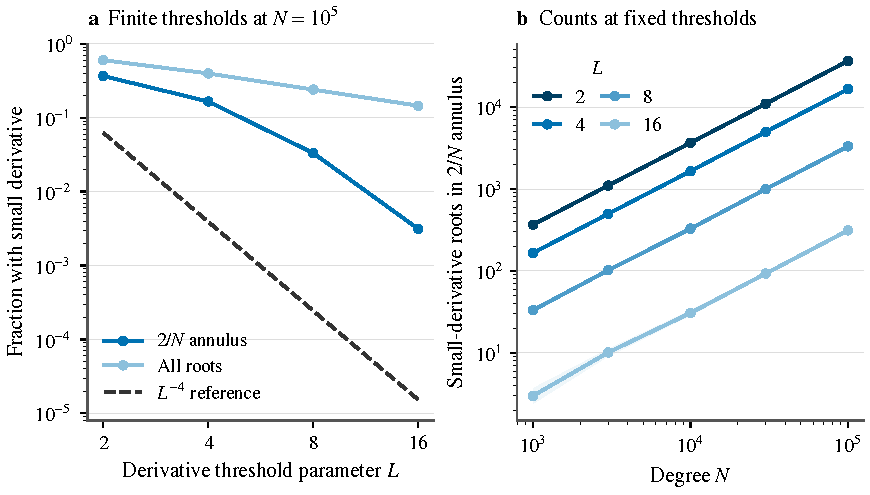
\includegraphics[width=\textwidth]{../numerics/publication/figures/small-derivative.pdf}
\caption{Zeros with small derivative, their fraction (a) and number (b)
over 77 sequences.}
\label{fig:small-derivative}
\end{figure}


\subsection{Bounds for appended tails}
\begin{lemma}[Appended tails]\label{lem:tails}
Let $K\ge2$, $N\ge\max\{4,K\}$ and $1\le m_{\max}\le N$. Set
\[
 \rho=1+K/N,\qquad g_m(z)=\sum_{k=N+1}^{N+m}\epsilon_kz^k,
 \qquad 0\le m\le m_{\max},
\]
and put
\[
 a=15e^{2K}\sqrt{m_{\max}\log N}.
\]
Outside an event of probability at most $N^{-10}$,
\[
 \max_{m\le m_{\max}}\sup_{|z|\le\rho}|g_m(z)|<a.
\]
\end{lemma}

\begin{proof}
As in the proof of Lemma~\ref{lem:second-derivative} for the second
derivative, we combine Hoeffding's inequality at the samples of the circle
$|z|=\rho$, a
deterministic bound on $g_m'$ between the samples, and the maximum
principle, now with the constants of the tails.

Note that the empty tail is identically zero.
We choose $\lceil N^3\rceil\le2N^3$ equally spaced samples on the boundary
circle. For every prefix, since $\rho\ge1$ and $k\le N+m\le2N$, we have
$\sum_{k=N+1}^{N+m}\rho^{2k}\le m\rho^{4N}\le m_{\max}e^{4K}$.
For a sample $z$ and $1\le m\le m_{\max}$, we apply Hoeffding's
inequality to
$\Re g_m(z)=\sum_{k=N+1}^{N+m}\epsilon_k\Re(z^k)$ and
$\Im g_m(z)=\sum_{k=N+1}^{N+m}\epsilon_k\Im(z^k)$, whose squared
coefficients are at most $|z|^{2k}=\rho^{2k}$. As in the proof of
Lemma~\ref{lem:second-derivative}, and since
$(2a/3)^2=100e^{4K}m_{\max}\log N$, we get
\begin{align*}
 \Prob\{|g_m(z)|\ge2a/3\}
 &\le\Prob\Bigl\{|\Re g_m(z)|\ge\frac{2a}{3\sqrt2}\Bigr\}
   +\Prob\Bigl\{|\Im g_m(z)|\ge\frac{2a}{3\sqrt2}\Bigr\}\\
 &\le4\exp\left[-\frac{(2a/3)^2}{4\sum_{k=N+1}^{N+m}\rho^{2k}}\right]
 \le4\exp\left[-\frac{(2a/3)^2}{4m_{\max}e^{4K}}\right]\\
 &=4\exp[-25\log N]=4N^{-25}.
\end{align*}
Since there are at most $2N^3$ samples and at most $m_{\max}\le N$
nonempty prefixes, there are at most $2N^4$ such pairs, and by the union
bound the probability that $|g_m(z)|\ge2a/3$ for one of them is at most
$(2N^4)(4N^{-25})=8N^{-21}\le N^{-10}$.
For the derivative we have the deterministic bound
\[
 \sup_{|z|\le\rho}|g_m'(z)|
 \le\sum_{k=N+1}^{N+m}k\rho^{k-1}
 \le m\cdot2N\cdot\rho^{2N}
 \le2Nm_{\max}e^{2K}.
\]
Since $N\ge K$, the circle $|z|=\rho$ has radius at most $2$ and length
at most $4\pi$, so that every
point of it lies within arc length $2\pi/N^3$ of a sample.
Therefore, since $m_{\max}\le\sqrt{m_{\max}}\sqrt N$ and
$4\pi<40\le5N^{3/2}\sqrt{\log N}$ for $N\ge4$, the error of
nearest-sample interpolation is at most
\[
 \frac{2\pi}{N^3}\cdot2Nm_{\max}e^{2K}
 =\frac{4\pi m_{\max}e^{2K}}{N^2}
 \le4\pi e^{2K}\sqrt{m_{\max}}\,N^{-3/2}
 <5e^{2K}\sqrt{m_{\max}\log N}
 =a/3.
\]
Outside this event, every point $\zeta$ of the circle of radius $\rho$ and
its nearest sample $z$ therefore satisfy, for $1\le m\le m_{\max}$,
\[
 |g_m(\zeta)|\le|g_m(z)|+\frac{4\pi m_{\max}e^{2K}}{N^2}
 <\frac{2a}3+\frac a3=a.
\]
By the maximum principle, the boundary bound extends to the disk.
Hence
$\max_{m\le m_{\max}}\sup_{|z|\le\rho}|g_m(z)|<a$
outside an event of probability at most $N^{-10}$, and this one event
controls every appended tail $g_m$ at once.
\end{proof}

